\documentclass[12pt]{article}

%packages go here!
\usepackage{anyfontsize}
\usepackage{tikz} %For drawing the cover page's background
\usepackage{graphicx}
\usepackage{titlesec}
\usepackage[a4paper,
	right=2cm,
	left=4.3cm,
	top=2.25cm, bottom=1.25cm]{geometry}
\usepackage[document]{ragged2e} %Left alignment
\usepackage{parskip} %Add an additional line after paragraphs
\usepackage{fancyhdr} %Put numbering on top
\usepackage{enumitem} %List handling
\usepackage{caption} %Caption handling
\usepackage{layout} %Printing out the layout for debugging
\usepackage[backend=biber, style=authoryear-icomp]{biblatex} %Bibliography
\providecommand\phantomsection{} %For putting unnumbered section in toc

%bibliography in latex's path:
\addbibresource{unilink.bib}

%Setting the font
\renewcommand{\rmdefault}{phv} % Arial
\renewcommand{\sfdefault}{phv} % Arial

%Enter parameters here: this is a mark
\newcommand\myauthor{Vo Dang Khoa (D5094; T5616SN)}
\newcommand\mytitle{TESLA, INC}
\newcommand{\subtitle}{}
\newcommand{\rpas}{Report}
\newcommand{\course}{Basics of Business Operations}

\linespread{1.5}

%Redefining maketitle
\renewcommand{\maketitle}{
\thispagestyle{empty}

\begin{center}

\fontsize{16}{19} \selectfont \myauthor

\vspace{20pt}

\MakeUppercase{\fontsize{24}{30} \selectfont \mytitle}

\vspace{5pt}

\fontsize{20}{25} \selectfont \subtitle

\vspace{20pt}

\fontsize{16}{19} \selectfont {\rpas \\ \course}

\vspace{20pt}

\the\year

%Adding the logo
\vspace{100pt}

\includegraphics{logo.jpg}

\end{center}

%Making the cover background
\tikz[remember picture,overlay] \node[inner sep=0pt] at (current page.center){

\includegraphics[width=\paperwidth,height=\paperheight]{coverbg.png}};
\clearpage
}

%Formatting The sections:
\titleformat{\section}
{\bfseries}
{\thesection}
{.17in}
{\MakeUppercase}

%The subsection:
\titleformat{\subsection}
{\bfseries}
{\thesubsection}
{.17in}
{}

%The subsubsection:
\titleformat{\subsubsection}
{\bfseries}
{\thesubsubsection}
{.17in}
{}

%Formatting the paragraphs
%Put new line between paragraphs
\setlength{\parskip}{\baselineskip}
%No indentation
\setlength{\parindent}{0pt}

%Content of the document
\begin{document}
%The cover page
%First we must clear up the margin
\newgeometry{
	right=2cm,
	left=2cm,
	top=4cm,
	bottom=2cm,
	}
{\maketitle}

%Table of content:
\thispagestyle{empty}
{\tableofcontents}

{\clearpage} %% old habits die hard ;-)

%Formatting the margin for the rest of the document
%(If 'restoregeometry' doesn't work then I have no other options":
\newgeometry{
	right=2cm,
	left=4.3cm,
	top=2.25cm,
	bottom=2.5cm,
	}

%Put numbering on top (i.e. the header)
\pagestyle{fancy}
\fancyhf{}
\chead{\thepage}
\renewcommand{\headrulewidth}{0pt} %No line please!

%Formatting lists:
\setlist[itemize]{leftmargin=.6in, nosep} %Vertical spacing of list paragraphs is none

%Caption handling:
\captionsetup[figure]{font=small, position=below}
\captionsetup[table] {font=small, positiona=above}












%The below line was marked!
%===========================================================================================================
%CONTENT GOES HERE!
\section{INTRODUCTION}
This is a report about the basics of Tesla’s operation.

\section{BASIC INFORMATION}
This chapter will give some basic information about Tesla, and why this company is interesting for me.

\subsection{Why I chose to investigate Tesla}
This is the company I’ve heard a lot about for many years and I think it is finally a convenient time to start learning about it. I am also quite interested in alternative energy sources and saving the environment.

\subsection{Basic information}
Tesla currently has 33,000 employees. The company’s products are automotive and energy storage. Tesla's headquarters are located in Palo Alto, California. It also has stores located in Canada, Europe, Asia and Australia.

The main market for all of Tesla’s car models is the United States. Norway is the largest overseas market for the Model S.

\section{HISTORY}

\subsection{The foundation}
The company was initially founded in 2003 by Martin Eberhard and Marc Tarpenning, although the company also considers Elon Musk, JB Straubel, and Ian Wright as its co-founders.

The founders were influenced to start the company after GM (General Motors) recalled and destroyed all of its EV1 electric cars in 2003. Tesla's early primary goal was to commercialize electric vehicles, starting with a premium sports car aimed at early adopters and then moving as rapidly as possible into more mainstream vehicles, including sedans and affordable compacts for the mass market, serving "as a catalyst to accelerate the day of electric vehicles" (\cite{bry16}).

\subsection{Main business development}
Tesla signed a production contract on July 11, 2005, with Group Lotus to produce "gliders" (complete cars minus powertrain). The contract ran through March 2011, but the two automakers extended the deal to keep the electric Roadster in production through December 2011 with a minimum number of 2,400 units

Musk led Tesla's Series B US\$13 million investment round. Musk co-led the third, US\$40 million round in May 2006. Tesla's third round included investment from prominent entrepreneurs including Google co-founders Sergey Brin and Larry Page. The fourth round in May 2007 added another US\$45 million and brought the total investments to over US\$105 million through private financing.

In October 2008, Musk became CEO and laid off an additional 25\% of Tesla's workforce.

By January 2009, Tesla had raised US\$187 million and delivered 147 cars. Musk had contributed US\$70 million of his own money to the company. Elon Musk owns a 20.8\% stake in the company as of March 2017. The prototype Model S was displayed at a press conference on March 26, 2009. 

In June 2009 Tesla was approved to receive US\$465 million in low-interest-bearing loans from the 2007 US\$8 billion Advanced Technology Vehicles Manufacturing Loan Program by the United States Department of Energy, while Ford got \$5.9 billion, and Nissan got \$1.6 billion. The funding came in 2010, and supported engineering and production of the Model S sedan, as well as the development of commercial powertrain technology. Tesla repaid the loan early and with \$12 million in interest in May 2013, and was the first of the automakers to repay.

On June 29, 2010, Tesla launched its initial public offering (IPO) on NASDAQ. 13,300,000 shares of common stock were issued to the public at a price of US\$17.00 per share. The IPO raised US\$226 million for the company.

\subsection{Most interesting business operations}

In June 2009 Tesla received US\$465 million in loans from the 2007 US\$8 billion Advanced Technology Vehicles Manufacturing Loan Program by the United States Department of Energy, while Ford got \$5.9 billion, and Nissan got \$1.6 billion. But it was the first company to repay the money.

The founders were influenced to start the company after GM (General Motors) recalled and destroyed all of its EV1 electric cars in 2003 (\cite{mu17}).

\section{EXTERNAL ENVIRONMENT}

\subsection{Economic environment}

I will now provide some information on the United States's economy. The source can be found next to the data.

\begin{itemize}
	\item{GDP (in 2016): 18.569 Trillion US\$ (From: World Bank)}
	\item{GDP per capita (in 2016): 57,466.787 US\$ (From: World Bank)}
	\item{Unemployment rate (in August 2017): 4.4\% (From: U.S. Bureau of Labor Statistics)}
	\item{Inflation rate (for 12 months ending in August 2017): 1.9\% (From: http://www.usinflationcalculator.com/inflation/current-inflation-rates/)}
	\item{Trade in 2017 (million US\$): Trade balance: -458,725.2 (a trade deficit); Total exports: 892,621.2; Total imports: 1,351,346.4 (From US' Census Bureau)}
\end{itemize}

Despite having heard of it before, I still find it rather interesting that the biggest economy in the world has a negative balance in trade. Even more interesting is that this deficit is due to consumer products and automobiles, and that the trading partner responsible for this is China. The unemployment is gradually declining, which is a good sign for the economy.

\subsection{Cultural Environment}

I will now discuss about cultural factors of the United States according to (\cite{hoUS}). First of all, there is a high degree of individualism and masculinity in the USA. That important factor plays a crucial role in advertising. Sometimes, showing that you are the best is more important than being actually the best, which is why Elon Musk, current CEO of Tesla decided to associate his brand name with the Roadster, a luxurious electric sportscar. This car showed to everyone that electric car can be as fast beautiful as any other traditional car.

The US scores below average on Uncertainty Avoidance. As a result, there is a fair degree of acceptance for new ideas and innovative product, something that Tesla also rely on.

However, Americans only score 26 on Long Term Orientation, which means that people don't change their mind easily and will continue to maintain time-honoured traditions and norms. Businesses also prefer to measure their performance on a short-term basis, something that Tesla does have to consider. Still, reality shows that Tesla has been doing well lately on the stock market, which means that investers are confident in the company's long term result.

\subsection{Political Environment}

According to (\cite{ko13}), Tesla wouldn't be a considered successful had it not been for the government's support, particularly from the Advanced Technology Vehicle Manufacturing program and President Obama. After the election of Donald Trump as president, many people worried that Tesla would lose federal support for its business. However, as I mentioned before, the company is still doing fine. \textcite{de16} went as far as saying: "It doesn't make sense for politics to turn against Elon Musk and Tesla", reasoning shutting down his company would result in a big economic loss.

\section{GLOBAL ENVIRONMENT AND INTERNATIONAL TRADE}

The top five trading partners of the US in the current year are China, Canada, Mexico, Japan and Germany (information was received from United States' Cencus Bureau). Seven out of fifteen trading partners are from Europe.

Tesla opened its first store in Europe in June 2009 in London's Knightsbridge district in the UK, followed by Munich in Germany in September. Tesla's European headquarters are in Amsterdam, the Netherlands.

Norway is the largest overseas market for Tesla's Model S, with 11,802 new units registered through October 2016 thanks to the country's comprehensive incentives for the adoption of pure electric cars. The Parliament of Norway set the goal to reach 50,000 zero emission vehicles by 2018. Among the existing incentives, all-electric cars and utility vans are exempt in Norway from all non-recurring vehicle fees, including purchase taxes, which are extremely high for ordinary cars, and 25\% VAT on purchase, together making electric car purchase price competitive with conventional cars.

\section{BUSINESS ETHICS AND CORPORATE SOCIAL RESPONSIBILITY}

\subsection{Tesla}

Tesla's written code of ethics can be found in (\cite{te10}).

Section "Compliance with Laws, Rules and Regulations" states, "Obeying the law, both in letter and in spirit, is the foundation on which this Company's ethical standards are built. All employees must respect and obey the laws of the cities, states and countries in which we operate. Although not all employees are expected to know the details of these laws, it is important to know enough to determine when to seek advice from supervisors, managers or other appropriate personnel."

Section "Conflicts of Interest" forbids employees from benefiting from things that conflict with the company's interest. An example may be working for another competing company.

Employees are not permitted to use or share confidential information for any purposes except the conduct of their business.

Section "Competition and Fair Dealing" states, "We seek to outperform our competition fairly and honestly. Stealing proprietary information, possessing trade secret information that was obtained without the owner's consent, or inducing such disclosures by past or present employees of other companies is prohibited."

Section "Discrimination and Harassment" says that the company values its diversity as a "tremendous asset". They will not tolerate any illegal discrimination or harassment of any kind.

Many more ethical statements can be found from the aforementioned document. The ones above are just what I find most significant.

According to (\cite{gr17}), Tesla has a corporate social responsibility strategy that relies on the nature of the business. For example, the company’s electric automobiles are widely viewed as an answer to the negative impacts of cars that use internal combustion engines. The following are Tesla’s stakeholders, arranged according to the company’s CSR prioritization:

\begin{itemize}
	\item{Communities (highest responsibility)}
	\item{Customers}
	\item{Employees}
	\item{Investors/Shareholders}
	\item{Governments}
\end{itemize}

About communities, Tesla directly satisfies the concerns of communities as significant stakeholders that determine brand image. One of the interests of this stakeholder group is to ensure that the natural environment is conserved or protected. Tesla’s electric automobile products address such interest. For example, communities are satisfied with the fact that these products are environmentally friendly because of zero emissions. Tesla also satisfies communities in terms of this stakeholder group’s interest in benefiting from advanced technologies. For example, in 2014, CEO Elon Musk announced that the company would allow other individuals and organizations to use its patents. This corporate social responsibility strategy directly benefits communities interested in using or developing technologies, emphasizing Tesla’s mission and vision statements.

For customers, Tesla seeks to improve product quality and pricing. For example, instead of continuing to buy batteries from Panasonic, Tesla plans to manufacture its own batteries to make its electric automobiles more affordable. Also, Tesla continues to expand its network of charging stations.

Tesla satisfies employees' interests through a competitive compensation strategy, as well as HR programs designed to enhance skills development and leadership development.

Tesla’s corporate social responsibility strategy addresses investors and shareholders' interests through long-term strategies that aim to transform the automotive market. For example, the company’s decision to allow other firms and individuals to use its technology patents is expected to increase market demand for electric vehicles, thereby creating growth opportunities for Tesla automobile sales.

The company satisfies Governments' interest through legal compliance and excellent sustainability, as well as business contribution to economic growth.

Although being the pioneer in the electric car market, Tesla does not just aim to build to build the best electric cars, they want to make the best cars. As evidence from their webpage:

\begin{itemize}
	\item{Quickest Acecleration.}
	\item{Longest Range.}
	\item{The Safest Cars Ever.}
\end{itemize}

Along with that, Tesla also "wanted to prove that people didn’t need to compromise to drive electric – that electric vehicles can be better, quicker and more fun to drive than gasoline cars." They "believes the faster the world stops relying on fossil fuels and moves towards a zero-emission future, the better."

\subsection{Google}

Google's ethic codes can be found on (\cite{go17}). "Don't be evil" is the theme emphasize in the company's ethic codes. It is not just about providing their users with unbiased information, but it's also about doing the right thing in generally "following the law, acting honorably, and treating co-workers with courtesy and respect." 

Google expect all of their employees and Board members to follow the Code. Moreover, they expect contractors, consultants and others who work for Google temporarily to follow the Code.

"We hold ourselves to a higher standard in how we treat users", said in the document. Google's responsibility for serving their users include:

\begin{itemize}
	\item{Integrity}
	\item{Usefulness}
	\item{Privacy, Security, and Freedom of Expression}
	\item{Responsiveness: recognize relevant user feedback and do something about it}
	\item{Take action: "Any time you feel our users aren’t being well-served, don’t be bashful - let someone in the company know about it."}
\end{itemize}

Regarding working relationship, the section "Support each other" includes:

\begin{itemize}
	\item{Equal Opportunity Employment}
	\item{Harassment, Discrimination, and Bullying: Google prohibits discrimination, harassment and bullying in any form – verbal, physical, or visual}
	\item{Drugs and alcohol: Consumption of alcohol is not banned. But any substance abuse is not permitted}
	\item{Safe workplace}
	\item{Dog policy: Google states clearly that it is a dog company}
\end{itemize}

In Google's "About Us" page (\cite{goa17}), they clearly emphasize their social responsibility with headlines like "Meet the researcher using Google Street View to help dementia patients with memory loss", "Studying the sea to make trash less toxic", "The hi-res future of anti pollution tech". We can see they are doing a really good job of marketing based on their social value.

\subsection{Microsoft}

Microsoft's codes of ethics can be found on (\cite{mssbc}) (the document is available in many languages). Some of the standards include:

\begin{itemize} 
	\item{Make good decisions: there are three steps: Pause, Think and Ask}
	\item{Speak up: there is no tolerance for relatiation}
	\item{Trust with out customer: honor privacy and secure data}
	\item{Trust with governments and communities}
	\item{Trust with each other}
	\item{Trust with investors}
\end{itemize}

I have some opinion on Microsoft's statements regarding trust with their customers. Since they have been really infamous for forcing Windows 10 down on Windows 7 and 8 laptops without users' permission (\cite{kle16}).

The company's corporate social responsibility can be found on (\cite{mscsr}). Some of the main things are:

\begin{itemize}
	\item{Empower every person and every organization}
	\item{Environmentally sustainable business practices}
	\item{Increase energy efficiency}
	\item{Minimize the impact of our waste}
	\item{Collaborate with others to tackle pressing environmental challenges}
\end{itemize}

On Microsoft's front webpage (www.microsoft.com), aside from their products you can also find headlines such as "Tackling water scarcity: Microsoft Cloud and Ecolab team up to find solutions". In this article you can find out about how Microsoft's cloud can help businesses reduce water consumption by collecting data, which is a nice example of how technology can change the world.

After reading about all these information on business ethics and corporate social responsibility, I have found out more about how companies and their customers can have a huge impact on societies and the environment. However, I am only convinced that I want to buy an electric car because I know that I can save the planet by doing so. About other things such as business ethics, I cannot trust the company's own guidelines (as mentioned above with Microsoft's case).

\section{MANAGING THE BUSINESS}

\subsection{Investigating Elon Musk}

In this section I will investigate Elon Musk, CEO of SpaceX and Tesla, based on (\cite{ry17}) and (\cite{to17})

Managing a huge business makes personally testing every candidate nearly impossible, but Musk interviewed every candidate himself. Generally, the best candidates get a call with a team manager, and then the best of the best must pass through Elon Musk himself. This fact shows that the entrepreneur puts a lot of effort into hiring the best people and not letting anyone he does not like into the company.

Musk does not require his candidate to have a college or even high school degree. He pointed out that really successful people such as Bill Gates or Steve Jobs all lack college degrees. "If you had a chance to hire them," he has said, "of course, that'd be a good idea."

Talent is important, but Musk also looks for candidates with a positive mindset. "It's very important to like the people you work with," he's said, "otherwise your job is going to be quite miserable."

Elon Musk does not like excessive meetings. Skyler Shuford, who used to work at Musk’s SpaceX company, recounted that he once heard a story about Musk telling someone in a meeting, “You haven’t said anything. Why are you in here?”

To sum it up, Elon Musk has what I call a "common sense" leadership style. He hires the best people and does not waste time.

\subsection{The mission, vision and strategy of Tesla}

Their goal is simple: "to accelerate the advent of sustainable transport by bringing compelling mass market electric cars to market as soon as possible." Their primary concern is not for the safety of the vehicle, which can be easily replaced, but for the safety of their customers.

Along with that goal comes the strategy. To achieve their first goal, the company initially released an expensive sportscar model, take that money to make cheaper cars, then eventually transition to selling average, mass market cars. How they plan to achieve complete safety can be found at (\cite{mu13}).

Tesla's vision is “to create the most compelling car company of the 21st century by driving the world’s transition to electric vehicles.” They are not interested in just being the best electric car company, they are interested in being the best car company of them all.

\subsection{Tesla's manager}

According to the page at (http://ir.tesla.com/management.cfm), these are the managers of Tesla:

\begin{itemize}
	\item{Elon Musk is the Chairman, Product Architect and CEO. Elon co-founded Tesla and continues to oversee the company's product strategy -- including the design, engineering and manufacturing of more and more affordable electric vehicles for mainstream consumers.}
	\item{JB Straubel is the Chief Technical Officer. As a co-founder of Tesla, JB has overseen the technical and engineering design of the vehicles, focusing on the battery, motor, power electronics, and high-level software sub-systems. Additionally, he evaluates new technology, manages vehicle systems testing, and handles technical interface with key vendors.}
	\item{Deepak Ahuja is the Chief Financial Officer. Deepak brings more than 20 years of global automotive financial experience to the Tesla team. As Chief Financial Officer, Deepak brings invaluable insight of a well-versed industry veteran to help Tesla become a leading automobile company in the world.}

\end{itemize}

\subsection{Recruitment for a managerial position}
Tesla is seeking a person for a position titled "Accessories NA Program Manager". The requirements are:

\begin{itemize}
	\item{BA/BS or the equivalent in experience is required; an MBA is preferred}
	\item{At least 3 years of relevant work experience - Experience launching new vehicle program/products in North America is a plus}
	\item{Experiences/Familiarity in aftermarket vehicle accessories and North America automobile market}
	\item{Excellent communication skills, both verbal and written}
	\item{Strong competency in MS office, Salesforce, and familiarity with Salesforce, Quickbase is a plus}
	\item{Works well under pressure and adapt to changes quickly}
	\item{can manage multiple priorities simultaneously}
	\item{Professional fluency in English/Spanish required; proficiency in other regional languages such as French is a big plus}
	\item{Excellent analytical and problem solving skills}
	\item{Ability to multitask in a fast moving environment and build a strong relationship with other business stakeholders}
\end{itemize}

\subsection{Corporate culture}

According to the webpage at (https://www.hofstede-insights.com/models/organisational-culture/), Organisational Culture is defined as the way in which members of an organisation relate to each other, their work and the outside world in comparison to other organisations. It can either enable or hinder an organisation’s strategy.

Tesla's own corporate culture is analyzed in (\cite{me17}). According to the article, Tesla identifies six main features of its organizational culture:

\begin{itemize}
	\item{Move Fast: Speed affects Tesla’s competitive advantage. This characteristic of the organizational culture highlights the importance of employees’ capability to rapidly respond to trends and changes in the market.}

	\item{Do the Impossible: In developing cutting-edge products, Tesla must ensure that its corporate culture encourages employees to think outside the box.}

	\item{Constantly Innovate: Innovation is at the heart of Tesla Motors, Inc. This feature of the organizational culture focuses on the continuous nature of innovation at the company.}

	\item{Reason from “First Principles”: CEO Elon Musk promotes reasoning from first principles, which involves identifying root factors to understand and solve problems.}

	\item{Think Like Owners: Tesla employs its organizational culture as a tool to maintain a mindset supportive of business development. The company wants its workers to think like they own the organization.}

	\item{We are ALL IN: Tesla Motors, Inc.’s organizational culture unifies employees into a team that works to improve the business.}
\end{itemize}

These characteristics of Tesla can be observed directly from the company's CEO Elon Musk himself. As described above, Elon Musk does not waste time, he selects the best people and his "First Principles" thinking is the foundation principle that helped him manage his business at both Tesla and SpaceX.

\section{ORGANISATIONAL STRUCTURES}

\subsection{Tesla's organizational design}

The organization structure of Tesla was discussed in (\cite{me17b}). According to the article, Tesla Motors, Inc. has an organizational structure that supports continuous business growth. Tesla’s organizational structure creates business capabilities that enable strong managerial control despite growing international operations.

Tesla has a functional organizational structure. The following characteristics are the most significant in the company's organizational structure:

\begin{itemize}
	\item{Global hierarchy (most important): This hierarchy involves management teams that control international operations, maintaining strict control over their operations.}
	\item{Global centralization: this organizational structure use one central group to control the entire company.}
	\item{Minimal regional divisions: different divisions are created to implement different strategies and marketing campaign accross different countries Tesla’s organizational structure has the following divisions mainly used for financial reporting:
	\begin{enumerate}
		\item{United States}
		\item{China}
		\item{Norway}
		\item{Other}
	\end{enumerate}
	}
\end{itemize}

Figure \ref{structpic} is a diagram describing the company's functional hierarchy.

\begin{figure}
	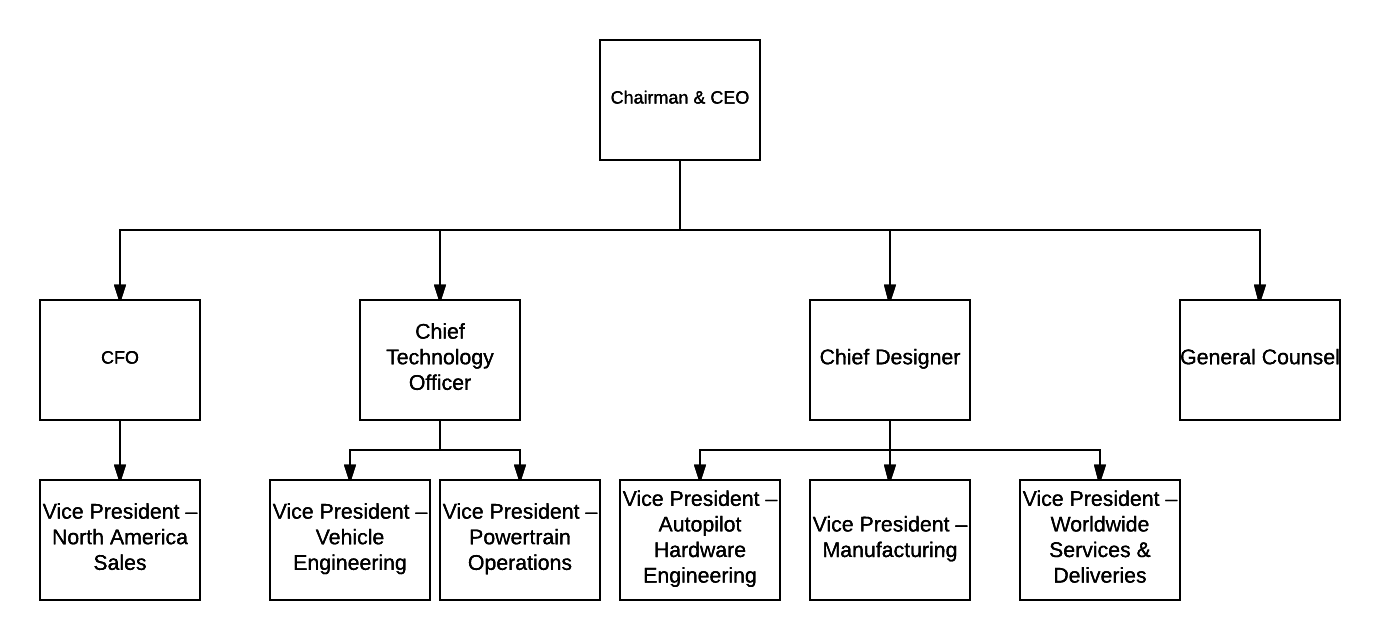
\includegraphics[width=\textwidth]{TeslaStruct.png}
	\caption{Tesla's organizational structure\label{structpic}}
\end{figure}

This organizational structure implies effective control of global operations. However, the lack of decentralization means that it can be hard for overseas branches to flexibly adjust their strategies. The success of overseas offices will rely strictly on the competence of the director board, which can potentially become a disadvantage of Tesla compared to local firms.

\subsection{Departmentalization examples}

Apart from Tesla, another company that adopts \textit{functional departmentalization} is Starbuck Coffee (\cite{me17c}). Starbuck's organizational structure is actually a matrix, which is a mixture of many different grouping methods. For example, the company has an HR department, a finance department and a marketing department with the CEO at the top.

Starbuck also uses \textit{product departmentalization} in its structure. For example, Starbucks has a division for coffee and related products, another division for baked goods, and another division for merchandise like mugs. With each division focusing on its product line, Starbuck can effectively manage its operations.

I unfortunately could not find any example company that uses \textit{process departmentalization} as one of its main division method. However, this method is similar to product departmentalization in a sense that different products involve different processes. However, division based on processes is more specific hence it is not often specified in the main departments.

%References, marked!
%---------------------------------------------------------------------------------------------------------------


%These two should always go together
\clearpage

\begingroup 
% NO more line spacing for references
\linespread{1}

% Set spacing between bibliography spacing
\setlength\bibitemsep{\baselineskip}

% NO more hanging indentation for bibliograpy
\setlength{\bibhang}{0pt}

\section*{REFERENCES}
\phantomsection
\addcontentsline{toc}{section}{REFERENCES}%

\printbibliography[heading=none]
\endgroup















\end{document}
